\section{Benchmark NIST-9 "Wave Front"}
\label{sec:bench-9}

This is a commonly used example for testing the performance of
adaptive refinement algorithms using a wave front and a singularity \cite{mitchell-1, mitchell-2}.
The solution has a sharp circular wave front in the interior of the
domain, with a singularity at the center of the circle.
The equation solved is the Poisson's equation.

\begin{equation} \label{wave-front}
-\Delta u = f
\end{equation}
in the domain $\Omega = (0, 1)^2$, equipped with Dirichlet boundary conditions
given by the exact solution. The exact solution is
$u(x, y) = tan^{-1}(\alpha (r - r_{0}))$,
where $r = \sqrt{(x - x_{loc})^{2} + (y - y_{loc})^{2}}$.
Here $(x_{loc}, y_{loc})$ is the center of the circular wave front,
$r_{0}$ is the distance from the wave front to the center of the circle,
and $\alpha$ gives the steepness of the wave front.
The right-hand side $f$ is calculated by inserting exact solution into (\ref{wave-front}).
The solution of NIST-9 with $\alpha = 50$, $(x_{loc}, y_{loc}) = (0.5, 0.5)$,
$r_{0} = 0.25$ is shown in Fig. \ref{fig:sln-nist09}.

\begin{figure}[!ht]
\centering
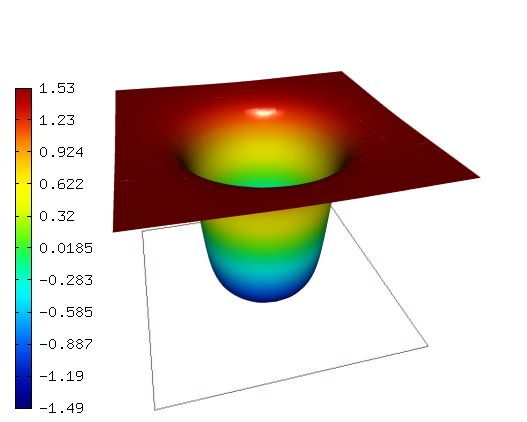
\includegraphics[height=5cm]{nist/nist-9/solution.png}
\caption{The solution to NIST-9 benchmark problem.}
\label{fig:sln-nist09}
\end{figure}

\begin{figure}[!ht]
\centering
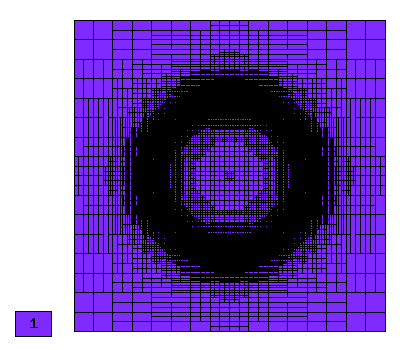
\includegraphics[height=3.7cm]{nist/nist-9/mesh_h1_aniso.png}
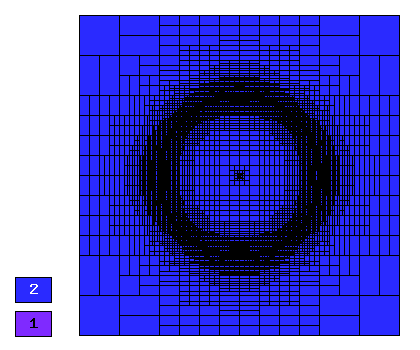
\includegraphics[height=3.7cm]{nist/nist-9/mesh_h2_aniso.png}
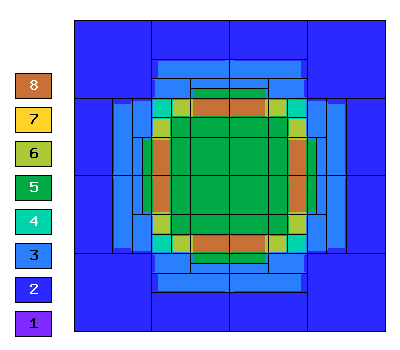
\includegraphics[height=3.7cm]{nist/nist-9/mesh_hp_aniso.png}
\caption{
Final mesh (left) with 46093 DOF and the resulting
relative error estimate in $H^1$-norm of 1.23973 \% for $h$-FEM with linear elements.
Final mesh (middle) with 4489 DOF and the resulting
relative error estimate in $H^1$-norm of 7.19928e-01 \% for $h$-FEM with quadratic elements.
Final mesh (right) with 1465 DOF and the resulting
relative error estimate in $H^1$-norm of 8.67667e-01 \% for $hp$-FEM with anisotropic refinements.}
\label{fig:nist-9-hp-aniso}
\end{figure}

%\begin{figure}[!ht]
%\centering
%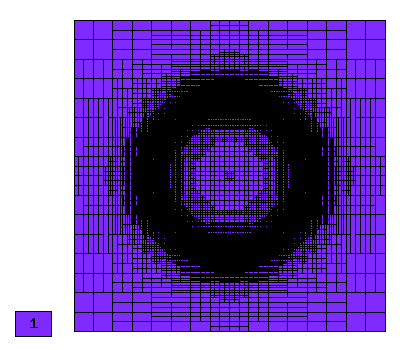
\includegraphics[height=5cm]{nist/nist-9/mesh_h1_aniso.png}\ \
%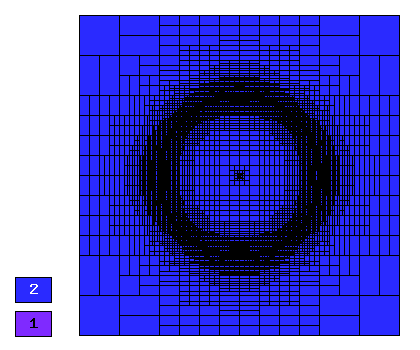
\includegraphics[height=5cm]{nist/nist-9/mesh_h2_aniso.png}
%\caption{Final mesh for $h$-FEM with linear and quadratic elements.}
%\label{fig:nist-9-h-aniso}
%\end{figure}

Figs. \ref{fig:nist-9-conv} compare all
three approaches to automatic adaptivity from the point
of view of DOF and CPU convergence.

\begin{figure}[!ht]
\centering
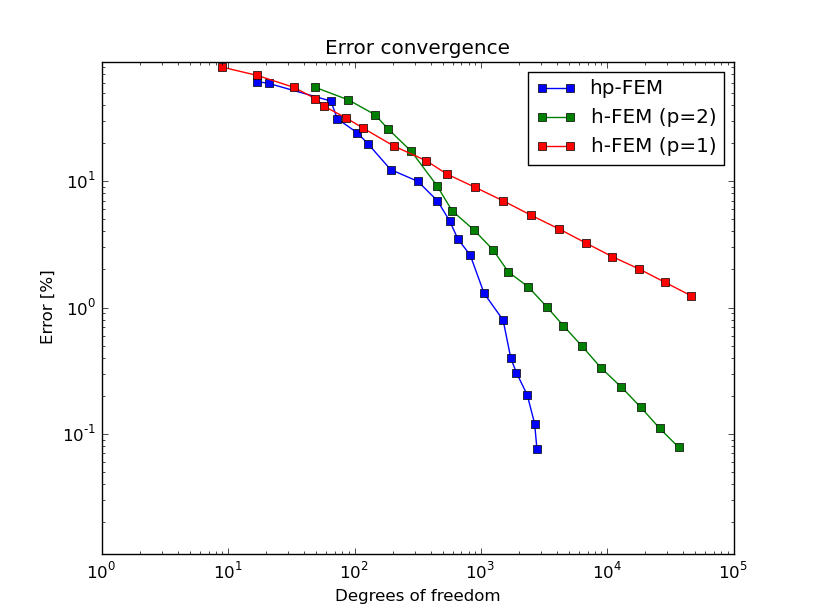
\includegraphics[height=5cm]{nist/nist-9/conv_dof_aniso.png}\ \
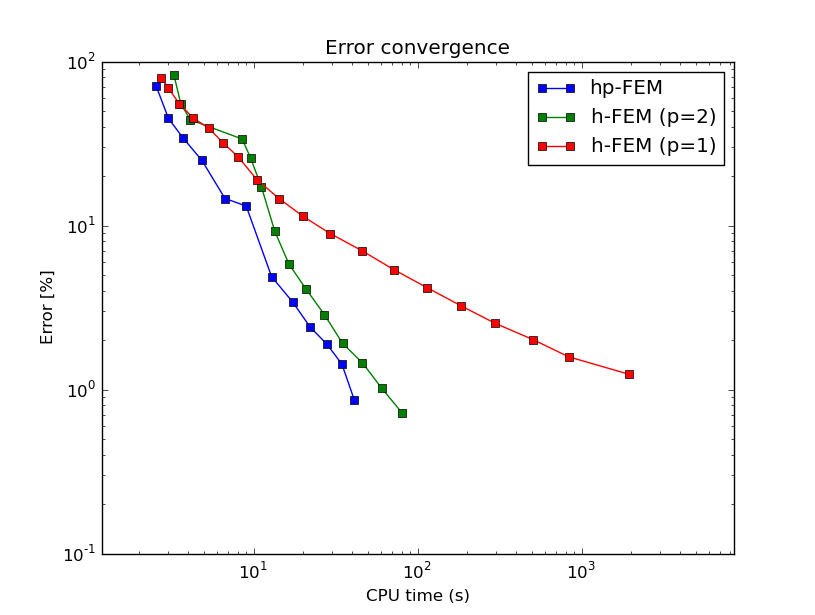
\includegraphics[height=5cm]{nist/nist-9/conv_cpu_aniso.png}
\caption{DOF and CPU time convergence graphs.}
\label{fig:nist-9-conv}
\end{figure}

